%%%%%%%%%%%%%%%%%%%%%%%%%%%%%%%%%%%%%%%%%
%
% CMPT 432
% Spring 2018
% Lab One
%
%%%%%%%%%%%%%%%%%%%%%%%%%%%%%%%%%%%%%%%%%

%%%%%%%%%%%%%%%%%%%%%%%%%%%%%%%%%%%%%%%%%
% Short Sectioned Assignment
% LaTeX Template
% Version 1.0 (5/5/12)
%
% This template has been downloaded from: http://www.LaTeXTemplates.com
% Original author: % Frits Wenneker (http://www.howtotex.com)
% License: CC BY-NC-SA 3.0 (http://creativecommons.org/licenses/by-nc-sa/3.0/)
% Modified by Alan G. Labouseur  - alan@labouseur.com
%
%%%%%%%%%%%%%%%%%%%%%%%%%%%%%%%%%%%%%%%%%

%----------------------------------------------------------------------------------------
%	PACKAGES AND OTHER DOCUMENT CONFIGURATIONS
%----------------------------------------------------------------------------------------

\documentclass[letterpaper, 10pt,DIV=13]{scrartcl} 

\usepackage[T1]{fontenc} % Use 8-bit encoding that has 256 glyphs
\usepackage[english]{babel} % English language/hyphenation
\usepackage{amsmath,amsfonts,amsthm,xfrac} % Math packages
\usepackage{sectsty} % Allows customizing section commands
\usepackage{graphicx}
\usepackage[lined,linesnumbered,commentsnumbered]{algorithm2e}
\usepackage{listings}
\usepackage{parskip}
\usepackage{lastpage}

\usepackage{tikz} %DFA drawings
\usetikzlibrary{automata,positioning}

\allsectionsfont{\normalfont\scshape} % Make all section titles in default font and small caps.

\usepackage{fancyhdr} % Custom headers and footers
\pagestyle{fancyplain} % Makes all pages in the document conform to the custom headers and footers

\fancyhead{} % No page header - if you want one, create it in the same way as the footers below
\fancyfoot[L]{} % Empty left footer
\fancyfoot[C]{} % Empty center footer
\fancyfoot[R]{page \thepage\ of \pageref{LastPage}} % Page numbering for right footer

\renewcommand{\headrulewidth}{0pt} % Remove header underlines
\renewcommand{\footrulewidth}{0pt} % Remove footer underlines
\setlength{\headheight}{13.6pt} % Customize the height of the header

\numberwithin{equation}{section} % Number equations within sections (i.e. 1.1, 1.2, 2.1, 2.2 instead of 1, 2, 3, 4)
\numberwithin{figure}{section} % Number figures within sections (i.e. 1.1, 1.2, 2.1, 2.2 instead of 1, 2, 3, 4)
\numberwithin{table}{section} % Number tables within sections (i.e. 1.1, 1.2, 2.1, 2.2 instead of 1, 2, 3, 4)

\setlength\parindent{0pt} % Removes all indentation from paragraphs.

\binoppenalty=3000
\relpenalty=3000

%----------------------------------------------------------------------------------------
%	TITLE SECTION
%----------------------------------------------------------------------------------------

\newcommand{\horrule}[1]{\rule{\linewidth}{#1}} % Create horizontal rule command with 1 argument of height

\title{	
   \normalfont \normalsize 
   \textsc{CMPT 432 - Spring 2018 - Dr. Labouseur} \\[10pt] % Header stuff.
   \horrule{0.5pt} \\[0.25cm] 	% Top horizontal rule
   \huge Lab Two  \\     	    % Assignment title
   \horrule{0.5pt} \\[0.25cm] 	% Bottom horizontal rule
}

\author{Juan S. Vasquez \\ \normalsize jvasquez1@marist.edu}

\date{\normalsize\today} 	% Today's date.

\begin{document}
\maketitle % Print the title

%----------------------------------------------------------------------------------------
%   start EXERCISE 3.3
%----------------------------------------------------------------------------------------
\section{Exercise 3.3}

\subsection{Regex for Finite Automata Examples}
1.) (ab*a)|(ba*b)\\
2.) a|a((bc|c)da)\textsuperscript{+}\\
3.) \displaystyle $\lambda$|(ab*c)
%----------------------------------------------------------------------------------------
%   end EXERCISE 3.3
%----------------------------------------------------------------------------------------

%----------------------------------------------------------------------------------------
%   start EXERCISE 3.4
%----------------------------------------------------------------------------------------
\section{Exercise 3.4}

\subsection{DFA One}
(a|(bc)*d)\textsuperscript{+}

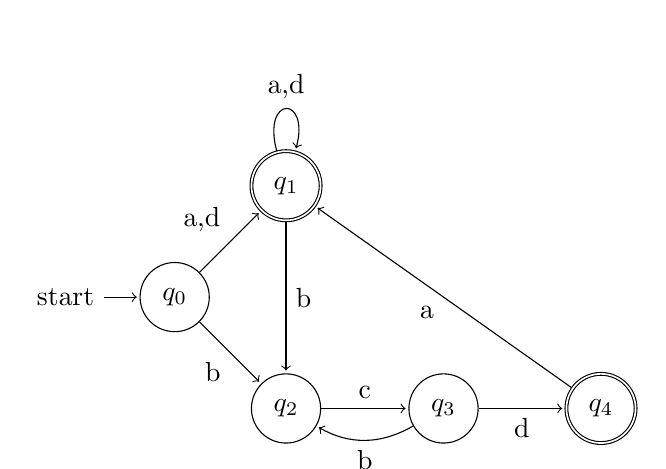
\begin{tikzpicture}[shorten >=1pt,node distance=2cm,on grid,auto]
% Here is where we draw each state and where 
% we want each state to be in relation to other states
   \node[state,initial] (q_0)   {$q_0$}; 
   \node[state,accepting] (q_1) [above right=of q_0] {$q_1$}; 
   \node[state] (q_2) [below right=of q_0] {$q_2$}; 
   \node[state] (q_3) [right=of q_2] {$q_3$};
   \node[state,accepting] (q_4) [right=of q_3] {$q_4$};
% Here is where we draw the paths between each state and specify curves, etc.
    \path[->] 
    (q_0) edge node {a,d} (q_1)
          edge node [swap] {b} (q_2)
    (q_1) edge node  {b} (q_2)
          edge [loop above] node {a,d} ()
    (q_2) edge node {c} (q_3) 
    (q_3) edge node [swap] {d} (q_4)
          edge [bend left] node {b} (q_2)
    (q_4) edge node {a} (q_1);
\end{tikzpicture}

\subsection{DFA Two}
((0|1)*(2|3)\textsuperscript{+})|0011

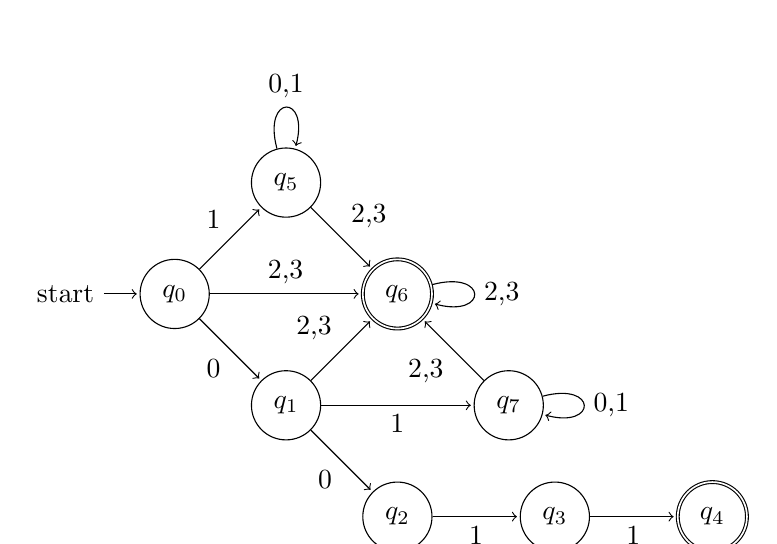
\begin{tikzpicture}[shorten >=1pt,node distance=2cm,on grid,auto] 
   \node[state,initial] (q_0)   {$q_0$}; 
   \node[state] (q_1) [below right=of q_0] {$q_1$}; 
   \node[state] (q_2) [below right=of q_1] {$q_2$}; 
   \node[state] (q_5) [above right=of q_0] {$q_5$};
   \node[state,accepting] (q_6) [below right=of q_5] {$q_6$};
   \node[state] (q_7) [below right=of q_6] {$q_7$};
   \node[state] (q_3) [right=of q_2] {$q_3$};
   \node[state,accepting] (q_4) [right=of q_3] {$q_4$};
    \path[->] 
    (q_0) edge node [swap] {0} (q_1)
          edge node {1} (q_5)
          edge node {2,3} (q_6)
    (q_1) edge node [swap] {0} (q_2)
          edge node {2,3} (q_6)
          edge node [swap] {1} (q_7)
    (q_2) edge node [swap] {1} (q_3)
    (q_3) edge node [swap] {1} (q_4)
    (q_5) edge [loop above] node {0,1} ()
          edge node {2,3} (q_6)
    (q_6) edge [loop right] node {2,3} ()
    (q_7) edge [loop right] node {0,1} ()
          edge node {2,3} (q_6);
\end{tikzpicture}

\subsection{DFA Three}
(a$Not$(a))*aaa

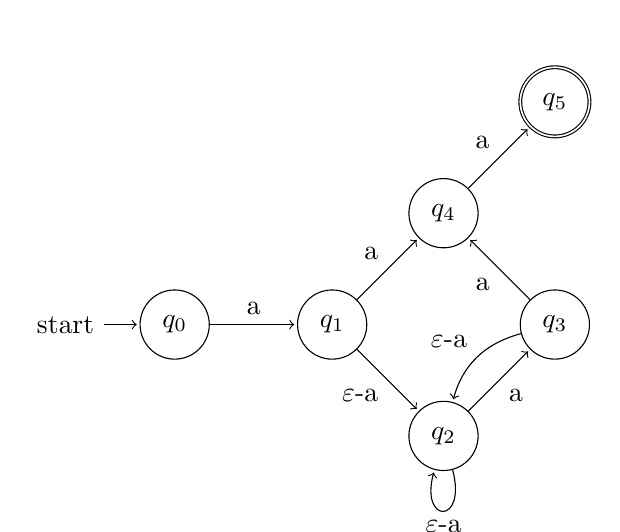
\begin{tikzpicture}[shorten >=1pt,node distance=2cm,on grid,auto] 
   \node[state,initial] (q_0)   {$q_0$}; 
   \node[state] (q_1) [right=of q_0] {$q_1$}; 
   \node[state] (q_2) [below right=of q_1] {$q_2$}; 
   \node[state] (q_3) [above right=of q_2] {$q_3$};
   \node[state] (q_4) [above right=of q_1] {$q_4$};
   \node[state,accepting] (q_5) [above right=of q_4] {$q_5$};
    \path[->] 
    (q_0) edge node {a} (q_1)
    (q_1) edge node {a} (q_4)
          edge node [swap] {$\varepsilon$-a} (q_2)
    (q_2) edge [loop below] node {$\varepsilon$-a} ()
          edge node [swap] {a} (q_3)
    (q_3) edge [bend right] node [swap] {$\varepsilon$-a} (q_2)
          edge node {a} (q_4)
    (q_4) edge node {a} (q_5);
\end{tikzpicture}
\pagebreak
%----------------------------------------------------------------------------------------
%   end EXERCISE 3.4
%----------------------------------------------------------------------------------------


%----------------------------------------------------------------------------------------
%   start EXERCISE 3.15
%----------------------------------------------------------------------------------------
\section{Exercise 3.15}

\subsection{NFA for Regex}
(ab*c)|(abc*)

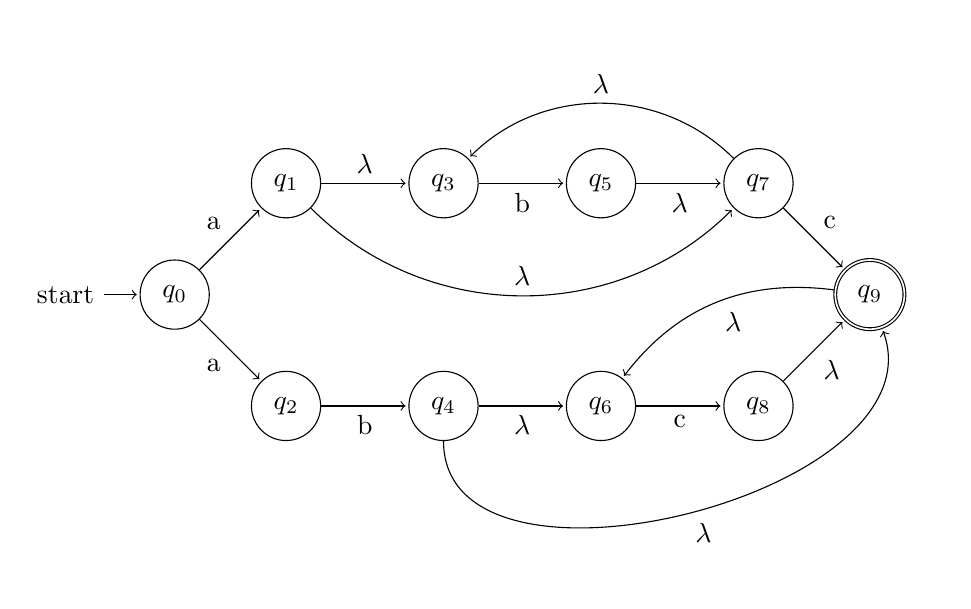
\begin{tikzpicture}[shorten >=1pt,node distance=2cm,on grid,auto] 
   \node[state,initial] (q_0)   {$q_0$}; 
   \node[state] (q_1) [above right=of q_0] {$q_1$}; 
   \node[state] (q_2) [below right=of q_0] {$q_2$}; 
   \node[state] (q_3) [right=of q_1] {$q_3$};
   \node[state] (q_4) [right=of q_2] {$q_4$};
   \node[state] (q_5) [right=of q_3] {$q_5$};
   \node[state] (q_6) [right=of q_4] {$q_6$};
   \node[state] (q_7) [right=of q_5] {$q_7$};
   \node[state] (q_8) [right=of q_6] {$q_8$};
   \node[state,accepting] (q_9) [above right=of q_8] {$q_9$};
    \path[->] 
    (q_0) edge node {a} (q_1)
          edge node [swap] {a} (q_2)
    (q_1) edge node {$\lambda$} (q_3)
          edge [out=315, in=225] node {$\lambda$} (q_7)
    (q_2) edge node [swap] {b} (q_4)
    (q_3) edge node [swap] {b} (q_5)
    (q_4) edge node [swap] {$\lambda$} (q_6)
          edge [out=270, in=290] node [swap] {$\lambda$} (q_9)
    (q_5) edge node [swap] {$\lambda$} (q_7)
    (q_6) edge node [swap] {c} (q_8)
    (q_7) edge node {c} (q_9)
          edge [out=135, in=45] node [swap] {$\lambda$} (q_3)
    (q_8) edge node [swap] {$\lambda$} (q_9)
    (q_9) edge [bend right] node {$\lambda$} (q_6);
\end{tikzpicture}

\subsection{DFA from previous NFA}
(ab*c)|(abc*)

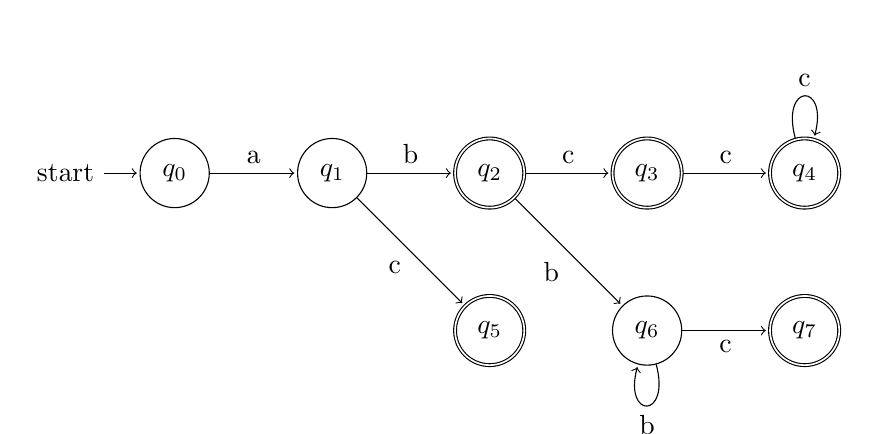
\begin{tikzpicture}[shorten >=1pt,node distance=2cm,on grid,auto] 
   \node[state,initial] (q_0)   {$q_0$}; 
   \node[state] (q_1) [right=of q_0] {$q_1$}; 
   \node[state,accepting] (q_2) [right=of q_1] {$q_2$}; 
   \node[state,accepting] (q_3) [right=of q_2] {$q_3$};
   \node[state,accepting] (q_4) [right=of q_3] {$q_4$};
   \node[state,accepting] (q_5) [below=of q_2] {$q_5$};
   \node[state] (q_6) [below=of q_3] {$q_6$};
   \node[state,accepting] (q_7) [below=of q_4] {$q_7$};
    \path[->] 
    (q_0) edge node {a} (q_1)
    (q_1) edge node {b} (q_2)
          edge node [swap] {c} (q_5)
    (q_2) edge node {c} (q_3)
          edge node [swap] {b} (q_6)
    (q_3) edge node {c} (q_4)
    (q_4) edge [loop above] node {c} (q_4)
    (q_6) edge node [swap] {c} (q_7)
          edge [loop below] node {b} (q_6)
    ;
\end{tikzpicture}
%----------------------------------------------------------------------------------------
%   end EXERCISE 3.15
%----------------------------------------------------------------------------------------


%----------------------------------------------------------------------------------------
%   start EXERCISE 3.3.4
%----------------------------------------------------------------------------------------
\section{Exercise 3.3.4}

\subsection{Case Insensitive Regex}
[Ss][Ee][Ll][Ee][Cc][Tt]

%----------------------------------------------------------------------------------------
%   end EXERCISE 3.3.4
%----------------------------------------------------------------------------------------

\end{document}
